% Apžvelgsime rekurentinio neuroninio tinklo, LSTM (angl. \textit{Long Short Term Memory}), veikimo principus.
% Rekurentinis neuroninis tinklas turi savyje atmintį(t.y. tinklas išvesdamas apskaičiuotas reikšmes atsižvelgia į tai kas vyko praeityje).

% Rekurentiniai neuroniniai tinklai, kitaip, nei paprasti neuroniniai tinklai turi grįštamuosius ryšius. Tai reiškia, kad šie tinklai apskaičiuodami naujas tinklo išvesties reikšmes atsižvelgia į praeitį. Šiam tikslui pasiekti rekurentiniai neuroniai tinklai savyje turi atmintį, kuri priklauso nuo prieš tai, kas vyko praeityje. Taip pat šis tinklas kaip įvesties reikšmes priema ne tik esamame laiko žingsnyje esamas įvesties reikšmes, bet ir praeito žingsnio išvesties reikšmes(būsenas), kas padeda tinklui tiksliau prognozuoti išvesties reikšmes priklausomai nuo praeities reikšmių.

% Šie rekurentiniai neuroniai tinklai savyje turi keturis paprastus neuroninius tinlus, kur kiekvienas iš jų atlieka savo paskirtį. Pirmasis neuroninis tinklas veikia, taip kad jo išvesties reikšmės nurodo kokią informaciją reikia pamiršti(t.y informaciją, kuri yra nereikšminga). Antrasis neuroninis tinklas kontroliuoja kiek naujos informacijos iš įvesties reikšmių reikia pridėti prie esamos informacijos. Trečiasis neuroninis tinklas dar papildomai pakoreguoja kiek naujos informacijos reikia išsisaugoti. Ketvirtasis neuroninis tinklas kontroliuoja kiek esamos informacijos turi būti perduodama apskaičiuojant naują tinklo išvesties reikšmę(būseną) ir kiek jos turi būti perduodama tolimesniem žingsniam.

% Reukurentinio neuroninio tinklo apmokymas vyksta į tinklą paduodant tam tikrus rinkinius duomenų. Tie rinkiniai sudaryti iš įvesties reikšmių ir reikšmių, kurias tikimasi gauti iš tinklo. Iš pradžių duomenys yra praleidžiami pro tinklą (angl. \textit{Feed forward}) ir poto atliekamas baudos funkcijos paklaidos mažinimas anti-gradientinio nusileidimo metodu (angl. \textit{Back Propogation}).
% Paminėti kad visi a priklauso nuo kiekvino svorio

\subsection{LSTM sandara}

Kuriamo neuroninio tinklo sandara bus tokia pati į literatūroje apžvelgtą LSTM rekurentinio neuroninio tinklo, tačiau detaliau aprašysiu visą tinklo veikimą ir naudojamus kintamuosius.

Sudarytas LSTM rekurintinis neuroninis tinklas. \ref{fig:rnnnn}

\begin{figure}[h!]
  \centering
\scalebox{0.4}{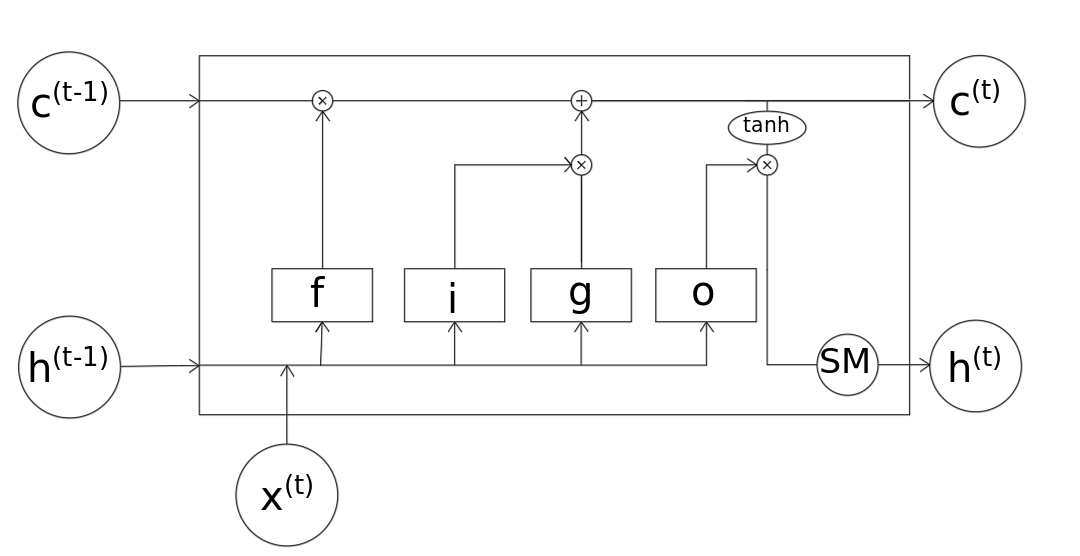
\includegraphics{images/lstmigwp2.png}}
\caption{Rekurentinis neuroninis tinklas.}
\label{fig:rnnnn}
\end{figure}


$M$ - išvesties ir atminties vektorių ilgis.\\
$I$ - įvesties reikšmių vektoriaus ilgis.\\
$V$ - neuroninių tinklų kiekis. \\
$L$ - nurodo atitinkamo neuroninio tinklo paskutinįjį sluoksnį.\\
$u$ - nuorodo skaičiuojamąjį tinklą.\\
$v$ - nuorodo bet kurį tinklą iš visų esamų (t.y. nėra skirtumo pagal, kurio tinklo reikšmės skaičiavimai yra atliekami).\\

\textbf{Atmintis}. Tinklas turi atmintį, kuri yra žymima $c_k^{(t)}$, čia c - vektorius, kuris saugo t laiko momentu gautas tinklo atminties reikšmes. Jo dydis yra M.\\

\textbf{Tinklo būsena}. Tinklas praeito žingsnio išvestį perduodą kaip naują būseną į dabartinį laiko momentą. Ji žymima $h_i^{(t)}$, čia h - vektorius, kuris saugo t laiko momentu gautas tinklo išvesties reikšmes. Jo dydis yra M. \\

\textbf{Įvesties reikšmės}. Esamuoju laiko momentu paduotos įvesties reikšmės žymimos $x_i^{(t)}$. Šio vektoriaus ilgis yra I. \\

\textbf{Neurono tarpinė reikšmė}. Į neuroną paduodamų sandaugų suma žymima $z_k^{u,l}$, čia z - nurodo u-ojo tinklo, l-ojo sluoksnio, k-ojo neurono sumą.\\

\textbf{Neurono reikšmė}. Neurono reikšmė pritaikius neurono tarpinei reikšmei aktyvacijos funkciją žymima $a_k^{(u,l)}$, čia a - nurodo u-ojo tinklo, l-ojo sluoksnio, k-ojo neurono reikšmę.\\

Neuroniai tinklai turi du svorių rinkinius:
\begin{enumerate}
  \item \textbf{Neuronus jungiantys svoriai}. Svoriai jungiantys dviejų gretimų sluoksnių neuronus žymimi $w_{ij}^{(v,s)}$, čia W - nurodo v-ojo tinklo svorį iš s-ojo sluoksnio i-ojo neurono į (s+1)-ojo sluoksnio j-ąjį neuroną.
  \item \textbf{Būsenų svoriai}. Svoriai jungiantys tinklo būseną su tinklų antrojo sluoksnio neuronais žymimi $w_{ij}^{(v)}$, čia W - nurodo v-ojo tinklo svorį iš $h_i^{(t)}$ būsenos į 2-ojo sluoksnio j-ąjį neuroną.\\
\end{enumerate}
% Neuronus jungiantys svoriai. Svoriai jungiantys dviejų gretimų sluoksnių neuronus žymimi $w_{ij}^{(v,s)}$, čia W - nurodo v-ojo tinklo svorį iš s-ojo sluoksnio i-ojo neurono į (s+1)-ojo sluoksnio j-ąjį neuroną. \\
%
% Būsenų svoriai. Svoriai jungiantys tinklo būseną su tinklų antrojo sluoksnio neuronais žymimi $w_{ij}^{(v)}$, čia W - nurodo v-ojo tinklo svorį iš $h_i^{(t)}$ būsenos į 2-ojo sluoksnio j-ąjį neuroną.\\

\textbf{Neuronų kiekiai sluoksniuose}. Vektorius saugantis neuroninių tinklų atitinkamų sluoksnių neuronų kiekis žymimas $K(u,l)$, čia K - nurodo u-ojo tinklo, l-ojo sluoksnio neuronų kiekį. \\

Tarpinės rekurentinio tinklo reikšmės žymimos $b_k^{(t)}$, čia b - nurodo tarpines k-asias išvesties reikšmes laiko momentu t.\\

\textbf{Tinklo baudos funkcija}. Tinklo paklaidą skaičiuojanti funkcija žymima $E^{(t)}$, čia E - tinklo baudos funkcijos reikšmė laiko momentu t.\\

\textbf{Kronekerio delta funkcija}. Funkcija, kuri palengvina aprašyti tam tikras formules $\delta_{u,v}$, čia funkcija, kuri gražina vienetą, jei kintamieji u ir v sutampa. \\

Keturi neuroniai tinklai. Visų tinklų veikimo principas yra vienodas, tačiau yra vienas skirtumas. Šie tinklai naudoja skirtingas aktyvacijos funkcijas.
\begin{enumerate}
  \item \textbf{Pirmasis}. Pamiršimo neuroninis tinklas. Žymimas - f. Jis naudoja Sigmoidinę aktyvacijos funkciją.
  \item \textbf{Antrasis}. Įvesties neuroninis tinklas. Žymimas - i. Jis naudoja Sigmoidinę aktyvacijos funkciją.
  \item \textbf{Trečiasis}. Įvesties moduliacijos neuroninis tinklas. Žymimas - g. Jis naudoja hiperbolinio tangento aktyvacijos funkciją.
  \item \textbf{Ketvirtasis}. Išvesties neuroninis tinklas. Žymimas - o. Jis naudoja Sigmoidinę aktyvacijos funkciją.
\end{enumerate}

Naudojamos aktyvacijos funkcijos:
\begin{enumerate}
  \item \textbf{Sigmoidinė} - $f(x) = \frac{1}{1+e^{-x}}$
  \item \textbf{Hiperbolinio tangento} - $f(x) = tanh(x)$
\end{enumerate}

Bet kurio neuroninio tinklo sandara.

\begin{figure}[h!]
  \centering
\scalebox{0.4}{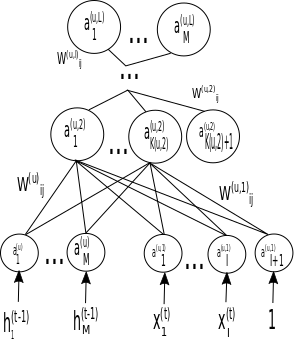
\includegraphics{images/drawing.png}}
\caption{Daugiasluoksnis neuroninis tinklas.}
\label{fig:drawing}
\end{figure}

% Rekurentinio neuroninio tinklo veikimo principas yra tas, kad


% Kiekvieno neuroninio tinklo sluoksnio neuronų kiekis yra vienetu didesnis, nei yra nurodyta tinklo topologijoje, dėl to, kad paskutinis atitinkamo sluoksnio neuronas yra pridedamas, kuris padeda greičiau apmokyti tinklą. Šis neuronas yra vadinamas "Bias" neuronu ir jo reikšmė visada yra lygi 1($a_{K(u,l)+1}^{(u,l)}=1$).

% Kiekvienas neuroninis tinklas turi po du svorių rinkinius. Vienas svorių rinkinys, kuris jungia praeito žingsnio tinklo išvesties reikšmes su atitinkamo neuroninio tinklo antrojo sluoksnio neuronais. Antrasis svorių rinkinys jungia visus likusius atitinkamo neuroninio tinklo neuronus tarpusavyje.

% Kiekvieno neuroninio tinklo atitinkamų dviejų gretimų sluoksnių neuronai yra apjungti svoriais. Kiekvienas žemesnio sluoksnio neuronas(įskaitant Bias neuroną) yra sujungtas su kiekvienu didesnio sluoksnio neuronu(išskyrus Bias neuroną) atitinkamu svoriu($w_{ij}^{u,l}$ svoris jungia $a_i^{(u,l)}$ neuroną su $a_j^{(u,l+1)}$ neuronu).

% Rekurentiniame neuroniniame tinkle esantys keturi neuroniai tinklai naudoja atitinkamas aktyvacijos funkcijas. Šiuo atveju pirmasis, antrasis ir ketvirtasis neuroniai tinklai naudoja logistinę sigmoidinę funkciją ($f(x) = \frac{1}{1+e^{-x}}$), o trečiasis tinklas naudoja hiperbolinio tangento funkciją($f(x) = tanh(x)$). Tinklo apmokymui yra naudojamos atitinkamų funkcijų išvestinės funkcijos.



  %
  % $h_i^{(t)}$ - vektorius, kuris saugo t laiko momentu gautas tinklo išvesties reikšmes.\\
  % $c_k^{(t)}$ - vektorius, kuris saugo t laiko momentu gautas tinklo atminties reikšmes.\\
  % $M$ - išvesties ir atminties vektorių ilgis.\\
  % $I$ - įvesties reikšmių vektoriaus ilgis.\\
  % $L$ - nurodo kiek sluoksnių yra atitinkamame tinkle.\\
  % $l$ - nurodo kiek neuronų yra atitinkamo tinklo l-ame sluoksnyje.\\
  % $w_{ij}^{(v,s)}$ - nurodo v-ojo tinklo svorį iš s-ojo sluoksnio i-ojo neurono į (s+1)-ojo sluoksnio j-ąjį neuroną.\\
  % $w_{ij}^{(v)}$ - nurodo v-ojo tinklo svorį iš $h_i^{(t)}$ būsenos į 2-ojo sluoksnio j-ąjį neuroną.\\
  % $a_k^{(u,l)}$ - nurodo u-ojo tinklo, l-ojo sluoksnio, k-ojo neurono reikšmę.\\
  % $z_k^{(u,l)}$ - nurodo u-ojo tinklo, l-ojo sluoksnio, k-ojo neurono sumą.\\
  % $K(u,l)$ - nurodo u-ojo tinklo, l-ojo sluoksnio neuronų kiekį. \\
  % $b_k^{(t)}$ - nurodo tarpines k-asias išvesties reikšmes.\\
  % $E^{(t)}$ - tinklo baudos funkcija.\\
  % $\delta_{u,v}$ - funkcija, kuri gražina vienetą, jei kintamieji u ir v sutampa. \\
